\chapter{Circuiti}
\subsection*{Elementi circuitali in parallelo}
Due o più elementi circuitali collegati in parallelo godono delle seguenti proprietà:
\begin{itemize}
\item{Ci si può spostare da un capo all'altro della configurazione attraversando un solo elemento.}
\item{Su ciascun elemento appare la stessa differenza di potenziale.}
\item{La corrente si suddivide tra i vari elementi.}
\end{itemize}

\subsection*{Elementi circuitali in serie}
Due o più elementi circuitali collegati in serie si godono delle seguenti proprietà:
\begin{itemize}
\item{Per passare da un capo all'altro della configurazione è necessario attraversare in successione tutti gli elementi.}
\item{La differenza di potenziale applicata agli estremi è pari alla somma delle differenze di potenziali su ciascun elemento.}
\item{Tutti gli elementi sono percorsi dalla stessa corrente.}
\end{itemize}

\section{Resistori}

\subsection{Resistori collegati in parallelo}
\begin{figure}[h!]
	\centering
    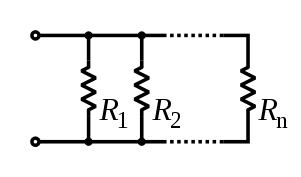
\includegraphics[scale=0.5]{Pictures/resistori-parallelo}
\end{figure}
Calcoliamo la resistenza equivalente di due resistori collegati in parallelo:
\begin{displaymath}\begin{aligned}
	i_1 = \frac{\Delta V}{R_1} \qquad i_2 = \frac{\Delta V}{R_2} \qquad i = i_1 + i_2 = \frac{\Delta V}{R}\\
    \frac{\Delta V}{R} = \frac{\Delta V}{R_1} + \frac{\Delta V}{R_2}\\
    \frac{1}{R} = \frac{1}{R_1} + \frac{1}{R_2}\\
\end{aligned}\end{displaymath}
Possiamo dimostrare, per induzione, che per $n$ resistori vale:
\begin{displaymath}
	\frac{1}{R} = \sum_{i=1}^n \frac{1}{R_i}
\end{displaymath}

\subsection{Resistori collegati in serie}
\begin{figure}[h!]
	\centering
    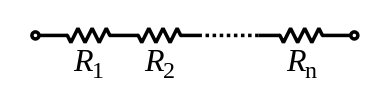
\includegraphics[scale=0.5]{Pictures/resistori-serie}
\end{figure}
Calcoliamo la resistenza equivalente $R$ di due resistori collegati in serie:
\begin{displaymath}\begin{aligned}
	\Delta V_1 = i \cdot R_1 \qquad \Delta V_2 = i \cdot R_2 \qquad \Delta V = \Delta V_1 + \Delta V_2 = i \cdot R \\ 
    i \cdot R = i \cdot R_1 + i\cdot R_2\\
    R = R_1 + R_2
\end{aligned}\end{displaymath}

Possiamo dimostrare, per induzione, che per $n$ resistori vale:
\begin{displaymath}
	R = \sum_{i=1}^n R_i
\end{displaymath}

\section{Condensatori}
Un condensatore piano è un sistema costituito da due superfici piane di materiale conduttore, aventi superficie $S$, poste a distanza $d$, in modo da costituire due piani paralleli.\\
Una superficie è caricata positivamente, l'altra negativamente.

\subsection{Campo elettrico all'interno di un condensatore}
All'interno del condensatore è presente un campo elettrico uniforme. Vediamo come calcolarlo.\\\\
Per il teorema di Gauss, una superficie piana carica genera un campo elettrico pari a:
\begin{displaymath}
	E = \frac{\sigma}{2 \cdot \epsilon_0}
\end{displaymath}
Poiché in un condensatore abbiamo due piani carichi sarà:
\begin{displaymath}
	E = 2 \cdot \frac{\sigma}{2 \cdot \epsilon_0} = \frac{\sigma}{\epsilon_0}
\end{displaymath}
Poiché $\sigma = \frac{Q}{S}$ possiamo scrivere:
\begin{displaymath}
	E = \frac{Q}{S \cdot \epsilon_0}
\end{displaymath}
Ricordiamo che il vettore campo elettrico è entrante per la lastra con carica negativa, e uscente per la piastra con carica positiva.\\
Possiamo dedurre che all’esterno delle due lastre il contributo al campo elettrico di ciascuna di esse fa si che il campo elettrico totale sia nullo; all’interno di esse, invece, il campo elettrico è doppio rispetto a quello generato da ogni singola armatura.

\subsection{Differenza di potenziale sulle armature del condensatore}
Utilizziamo la definizione di energia potenziale (in cui il punto A rappresenta una delle armature e il punto B rappresenta l'altra):
\begin{displaymath}
	\Delta V = \int_A^B \vec{E} \cdot d\vec{s}
\end{displaymath}
Poiché i versori che indicano la direzione di $\vec{E}$ e $d\vec{S}$ sono paralleli, il loro prodotto scalare è pari a 1, quindi:
\begin{displaymath}
	\Delta V = \frac{Q}{S \cdot \epsilon_0} \cdot d
\end{displaymath}

\subsection{Capacità di un condensatore piano}
La capacità di un condensatore è il rapporto tra la carica che può immagazzinare e la differenza di potenziale sulle armature.\\
Si tratta di una costante che dipende soltanto dalle caratteristiche fisiche e geometriche del condensatore.
\begin{displaymath}
	C = \frac{Q}{\Delta V} = Q \cdot \frac{S \cdot \epsilon_0}{Q \cdot d} = \frac{S \cdot \epsilon_0}{d} 
\end{displaymath}

\subsection{Cosa accade all'esterno del condensatore}
Come abbiamo detto nel paragrafo 4.2.1, il campo elettrico all'esterno del condensatore è nullo. Ciò implica che sia nullo anche il potenziale.

\subsection{Carica e scarica del condensatore}
\subsubsection{Processo di carica}
La carica si accumula sulle armature del condensatore quando viene applicata una differenza di potenziale $\Delta V = \epsilon$
\begin{displaymath}\begin{aligned}
	Q(t) = Q_{MAX} \cdot (1- e^{\frac{-t}{RC}})\\
    Q(t) = C \cdot \Delta V \cdot (1- e^{\frac{-t}{RC}})
\end{aligned}\end{displaymath}
\begin{itemize}
	\item{$t < 0$: condensatore scarico}
    \item{$t \rightarrow 0$: condensatore in carica 
    	\begin{displaymath}\begin{aligned}
            Q(t) = Q_{MAX} \cdot (1- e^{\frac{-t}{RC}}) = 
            Q_{MAX} \cdot (1- e^{\frac{-0}{RC}}) = 
            Q_{MAX} \cdot (1- 1) = 0
    	\end{aligned}\end{displaymath}}
    \item{$t \rightarrow \infty$: condensatore carico a regime
      \begin{displaymath}\begin{aligned}
              \Delta V = \epsilon\\
              Q(t) = Q_{MAX} (1- e^{\frac{-\infty}{RC}}) = 
              Q_{MAX} = C \cdot \epsilon
          \end{aligned}\end{displaymath}}
\end{itemize}

\subsubsection{Processo di scarica}
La carica accumulata sulle armature viene rilasciata, generando una $\Delta V = \epsilon$.
\begin{displaymath}\begin{aligned}
	Q(t) = Q_{MAX} \cdot (e^{\frac{-t}{RC}})\\
    Q(t) = C \cdot \Delta V \cdot (e^{\frac{-t}{RC}})
\end{aligned}\end{displaymath}
\begin{itemize}
	\item{$t < 0$: condensatore carico
    	\begin{displaymath}\begin{aligned}
    		Q(t) = Q_{MAX} (e^{\frac{-0}{RC}}) = Q_{MAX} = C \cdot \epsilon
    	\end{aligned}\end{displaymath}}
    \item{$t \rightarrow 0$: condensatore inizia a scaricarsi 
    	\begin{displaymath}\begin{aligned}
            Q(t) = Q_{MAX} \cdot (e^{\frac{-t}{RC}})\\
    Q(t) = Q_{MAX} \cdot (e^{\frac{-0}{RC}}) = Q_{MAX} = C \cdot \epsilon
    	\end{aligned}\end{displaymath}
        Il condensatore si comporta come un generatore avente una fem pari a 
        \begin{displaymath}
        	\epsilon = \frac{Q_{MAX}}{C}
        \end{displaymath}}
    \item{$t \rightarrow \infty$: condensatore scarico
      	\begin{displaymath}\begin{aligned}
        	Q(t) = Q_{MAX} \cdot (e^{\frac{-\infty}{RC}}) = 0
         \end{aligned}\end{displaymath}}
\end{itemize}

\subsection{Condensatori collegati in parallelo}
\begin{figure}
	\centering
    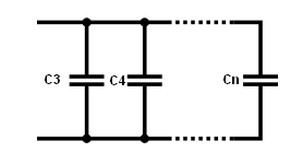
\includegraphics[scale = 0.7]{Pictures/condensatori-parallelo}
\end{figure}
Calcoliamo la capacità equivalente $C$ di due condensatori collegati in serie:
\begin{displaymath}\begin{aligned}
	q_1 = C_1 \cdot \Delta V \qquad q_2 = C_2 \cdot \Delta V \qquad q = q_1 + q_2 = C \cdot \Delta V\\
    C \Delta V = C_1 \Delta V + C_2 \Delta V\\
    C = C_1 + C_2
\end{aligned}\end{displaymath}
Possiamo dimostrare, per induzione, che per $n$ condensatori vale:
\begin{displaymath}
	C = \sum_{i=1}^n C_i
\end{displaymath}

\subsection{Condensatori collegati in serie}
\begin{figure}[h!]
	\centering
    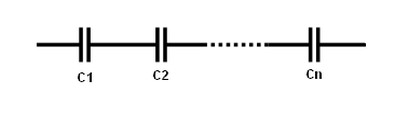
\includegraphics[scale = 0.8]{Pictures/condensatori-serie}
\end{figure}
Calcoliamo la capacità equivalente di due condensatori collegati in parallelo:
\begin{displaymath}\begin{aligned}
	\Delta V_1 = \frac{q}{C_1} \qquad \Delta V_2 = \frac{q}{C_2} \qquad
    \Delta V = \Delta V_1 + \Delta V_2 = \frac{q}{C}\\
    \frac{q}{C} = \frac{q}{C_1} + \frac{q}{C_2}\\
    \frac{1}{C} = \frac{1}{C_1} + \frac{1}{C_2}
\end{aligned}\end{displaymath}

Possiamo dimostrare, per induzione, che per $n$ resistori vale:
\begin{displaymath}
	\frac{1}{C} = \sum_{i=1}^n \frac{1}{C_i}
\end{displaymath}